\documentclass{article}
\usepackage[utf8]{inputenc}
\usepackage{tikz}
\usetikzlibrary{positioning}
\usetikzlibrary{shapes}

\begin{document}

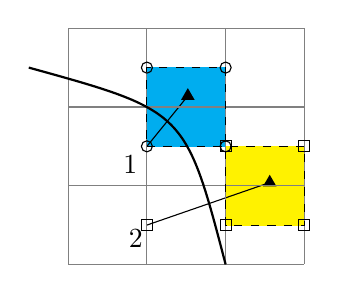
\begin{tikzpicture}
%blue node
\filldraw[cyan] (-0.5,0) rectangle (0.5,1);%shade
\node[fill=black,regular polygon, regular polygon sides=3,inner sep=1.0pt] at (0.02,0.64) {};%IP
\draw[black, thin] (-0.5,0) -- (0.02, 0.64);%line
%yellow node
\filldraw[yellow] (0.5,-1) rectangle (1.5,0);%shade
\node[fill=black,regular polygon, regular polygon sides=3,inner sep=1.0pt] at (1.06,-0.46) {};%IP
\draw[black, thin] (-0.5,-1) -- (1.06, -0.46);%line
%grid
%horizontal
\draw[gray, thin] (-1.5,1.5) -- (1.5,1.5);
\draw[gray, thin] (-1.5,0.5) -- (1.5,0.5);
\draw[gray, thin] (-1.5,-0.5) -- (1.5,-0.5);
\draw[gray, thin] (-1.5,-1.5) -- (1.5,-1.5);
%vertical
\draw[gray, thin] (-1.5,1.5) -- (-1.5,-1.5);
\draw[gray, thin] (-0.5,1.5) -- (-0.5,-1.5);
\draw[gray, thin] (0.5,1.5) -- (0.5,-1.5);
\draw[gray, thin] (1.5,1.5) -- (1.5,-1.5);
%outline
\draw[black, thin, dashed] (-0.5,0) -- (0.5,0) -- (0.5,1) -- (-0.5,1) -- cycle;
\draw[black, thin, dashed] (1.5,0) -- (0.5,0) -- (0.5,-1) -- (1.5,-1) -- cycle;
%blue stencil
\draw [black] (-0.5,1) circle (2pt);
\draw [black] (0.5,1) circle (2pt);
\draw [black] (0.5,0) circle (2pt);
\draw [black] (-0.5,0) circle (2pt) node[anchor=north east] {1};

%yellow stencil
\draw [black] ([xshift=-2pt,yshift=-2pt]0.5,0) rectangle ++(4pt,4pt);
\draw [black] ([xshift=-2pt,yshift=-2pt]1.5,0) rectangle ++(4pt,4pt);
\draw [black] ([xshift=-2pt,yshift=-2pt]0.5,-1)rectangle ++(4pt,4pt);
\draw [black] ([xshift=-2pt,yshift=-2pt]1.5,-1) rectangle ++(4pt,4pt);
\draw [black] ([xshift=-2pt,yshift=-2pt]-0.5,-1) rectangle ++(4pt,4pt) node[anchor=north east] {2};
%body
\draw[black, thick] (0.5,-1.5) .. controls (-0.01,0.45) .. (-2,1);

\end{tikzpicture}


\end{document}
